%%%%%%%%%%%%%%%%%%%%%%%%%%%%%%%%%%%%%%%%%%%%%%%%%%%%%%%%%%%%%%%%%%%%%%%%%%%%%%%%
%2345678901234567890123456789012345678901234567890123456789012345678901234567890
%        1         2         3         4         5         6         7         8

\documentclass[letterpaper, 10 pt, conference]{ieeeconf}  % Comment this line out if you need a4paper

%\documentclass[a4paper, 10pt, conference]{ieeeconf}      % Use this line for a4 paper

\IEEEoverridecommandlockouts                              % This command is only needed if 
                                                          % you want to use the \thanks command

\overrideIEEEmargins                                      % Needed to meet printer requirements.

% See the \addtolength command later in the file to balance the column lengths
% on the last page of the document

% The following packages can be found on http:\\www.ctan.org
%\usepackage{graphics} % for pdf, bitmapped graphics files
\usepackage{epsfig} % for postscript graphics files
%\usepackage{mathptmx} % assumes new font selection scheme installed
%\usepackage{times} % assumes new font selection scheme installed
%\usepackage{amsmath} % assumes amsmath package installed
%\usepackage{amssymb}  % assumes amsmath package installed

\title{\LARGE \bf
Humanoid robot AR-600
}


\author{Evgenii Koriagin$^{1}$, Sergey Oreshkov$^{2}$, Vladislav
Sychkov$^{3}$, Oleg Tolstel$^{4}$% <-this
% % stops a space \thanks{*This work was not supported by any organization}% <-this % stops a
% space
\thanks{$^{1}$Evgenii Koriagin is researcher at Intelligent Robotics
Laboratory, I.Kant Baltic Federal University, Kaliningrad, Russia {\tt\small
ekoryagin@kantiana.ru}}%
\thanks{$^{2}$Sergey Oreshkov is researcher at Intelligent Robotics
Laboratory, I.Kant Baltic Federal University, Kaliningrad, Russia {\tt\small
soreshkov@kantiana.ru}}%
\thanks{$^{3}$Vladislav Sychkov is CEO of Android Techniques, Magnitogorsk,
Russia {\tt\small info@rusandroid.com}}%
\thanks{$^{4}$Oleg Tolstel is head of Intelligent Robotics
Laboratory, I.Kant Baltic Federal University, Kaliningrad, Russia {\tt\small
otolstel@kantiana.ru}}%
}


\begin{document}



\maketitle
\thispagestyle{empty}
\pagestyle{empty}


%%%%%%%%%%%%%%%%%%%%%%%%%%%%%%%%%%%%%%%%%%%%%%%%%%%%%%%%%%%%%%%%%%%%%%%%%%%%%%%%
\begin{abstract}

This article describes the hardware design and some of the software of
autonomous humanoid robot AR-600. It is a full-sized humanoid robot that can be
used in human-centered environment. 

\end{abstract}


%%%%%%%%%%%%%%%%%%%%%%%%%%%%%%%%%%%%%%%%%%%%%%%%%%%%%%%%%%%%%%%%%%%%%%%%%%%%%%%%
\section{INTRODUCTION}

One of the main applications for robots in nearest future would be to replace
(or assist) humans in dangerous situations and hazardous environments. Another
important niche for robots is to help humans in their everyday life: assist in
study and research, in housekeeping, in the kitchen, elderly care, etc.

AR-600 (fig. \ref{img:ar600}), developed by Russian company Android Techniques
\cite{c1}, is aimed to be a multitasking antropomorphic robotic platform that
can interact with humans and operate in human infrastructure. 
   
It was designed to have a size of a 14-16 years old teenager. And that was done
by purpose. Robot that is a bit smaller than a typical human can be treated
with all respect like a younger brother who's trying to help in everyday
routine. Looking at the robot from above will lead to a better attitude while
communicating with it. 
  
\begin{figure} [thpb]
      \centering
      \framebox{
      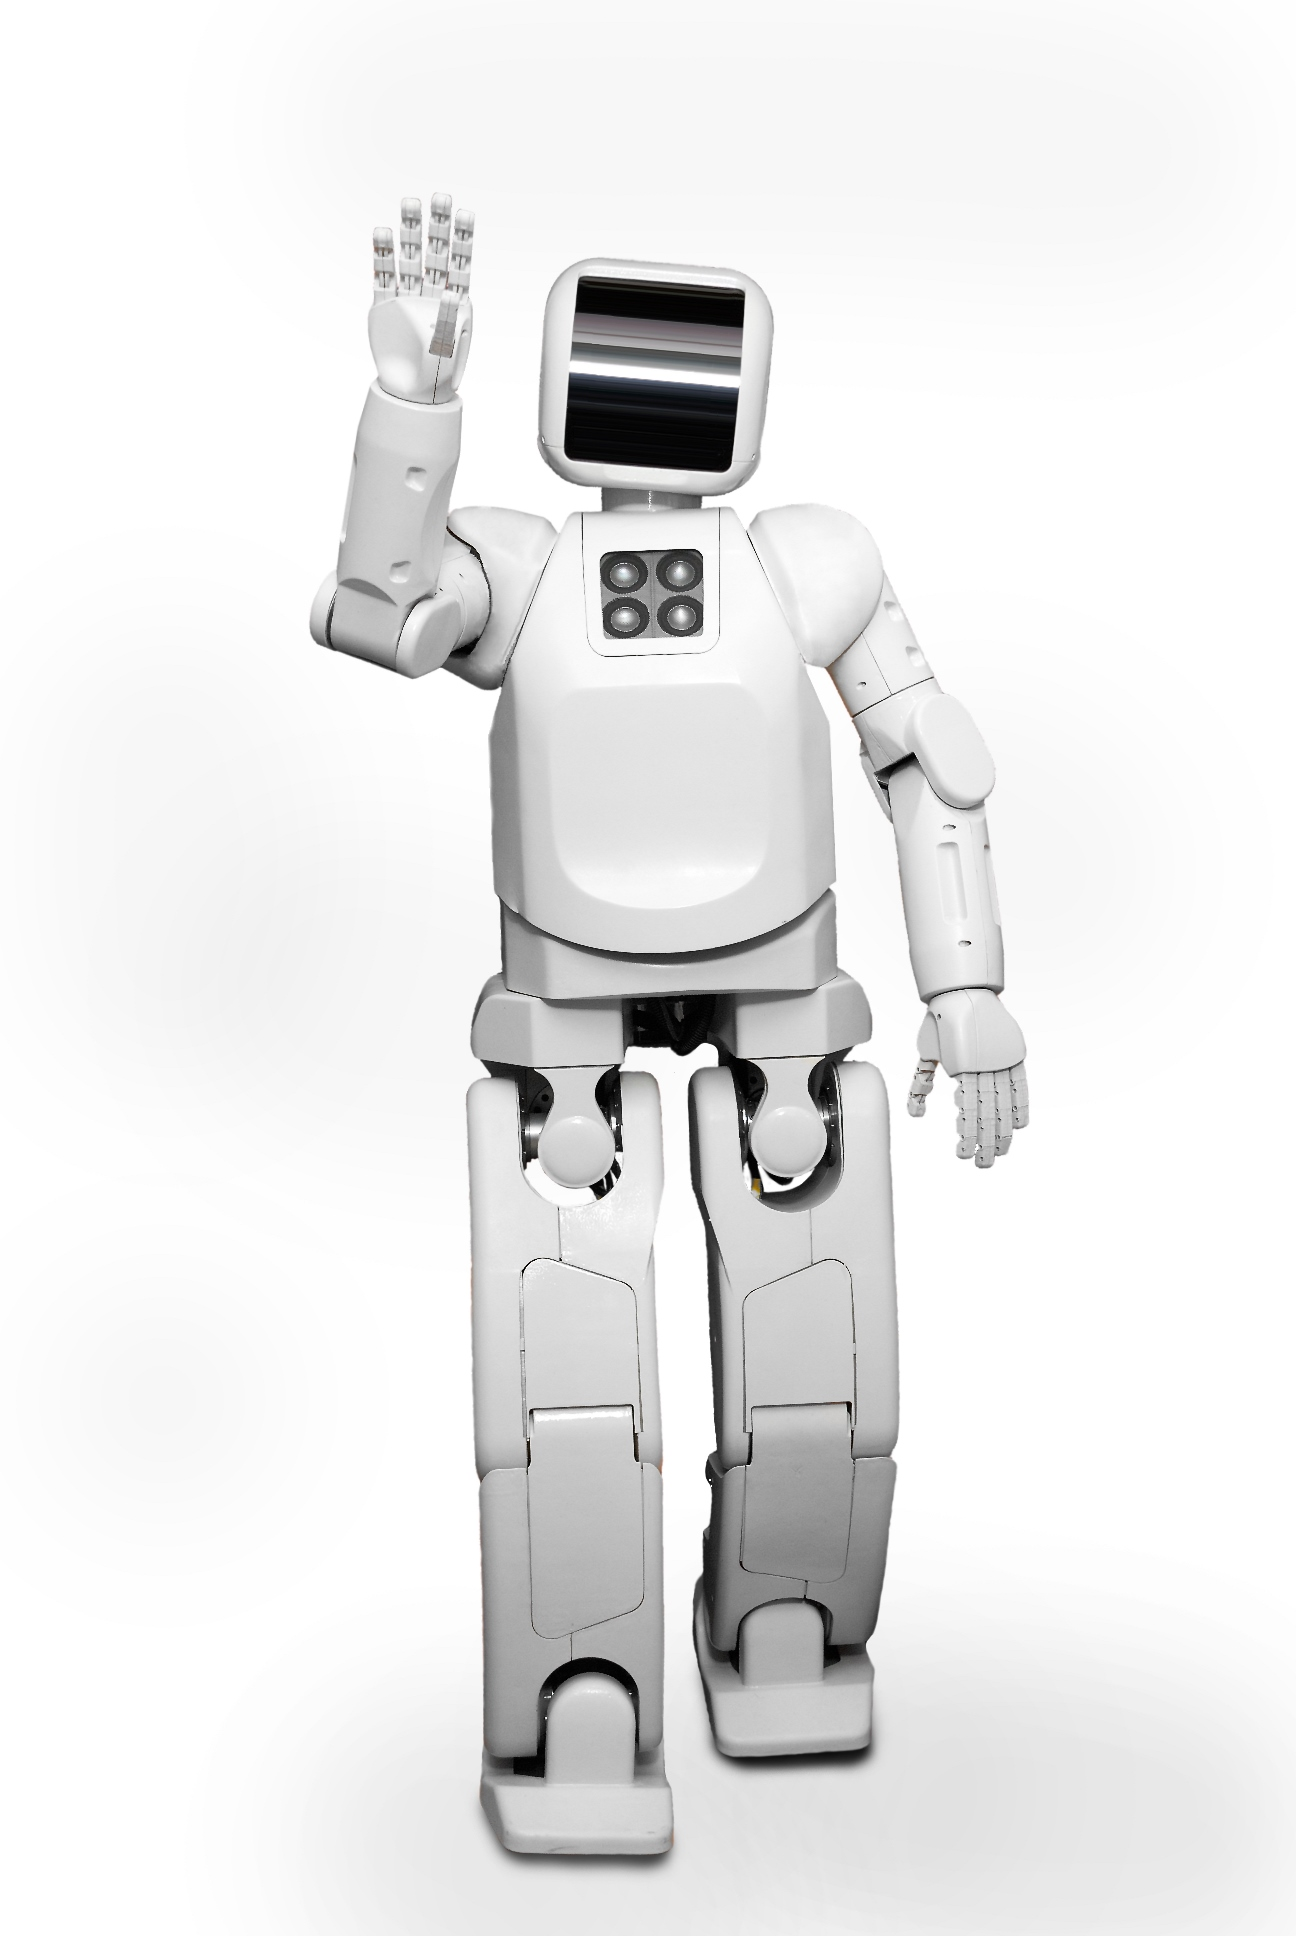
\includegraphics[scale=0.2]{ar600}}
      \caption{Antropomorphic robot AR-600.}
      \label{img:ar600}
\end{figure}


\begin{figure} [thpb]
      \centering
      \framebox{
      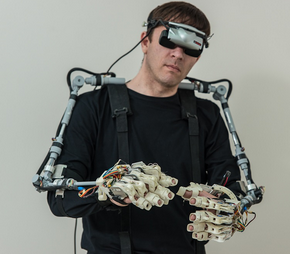
\includegraphics[scale=0.8]{suit}}
      \caption{Mimicking device for the robot.}
      \label{img:suit}
\end{figure}

Abilities of robots to accomplish certain tasks autonomously relies mostly on
a high level software that implements all the best from the field of artificial
intelligence. The other way that allows to use robots now is to make them mimic
our moves like avatars. Our AR-600 robot can be controlled by a developed
mimicking device (fig. \ref{img:suit}). It sends joint angles to robot and
gets back force feedback and video stream. With this ``suit'' on an
operator can naturally control the upperbody of the robot and use it to manipulate tools in uninhabitable or hazardous environments (e.g. welding or screwing).

AR-600 is already used in 6 Russian universities as a robotics research
platform. Some of the research topics are object grasping and bipedal walking.

This paper describes specifications of the robot, software developed so far and
some future work.
\section{SPECIFICATIONS OF AR-600}

Weight of robot is about 55 kilograms.
The overview of kinematic structure is shown in Fig.\ref{img:kinematic}, list of
DOF is presented in Table 1.
 \begin{figure}[thpb]
      \centering
      \framebox{
        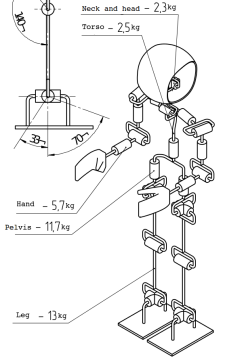
\includegraphics[scale=.5]{panview}
      }
      \caption{Kinematic scheme}
      \label{img:kinematic}
   \end{figure}
 

\begin{table}[thpb]
    \caption{Joints degrees of freedom}
    \label{table}
    \begin{center}
    \begin{tabular}{c | c c c}
        & degree of freedom & range of motion & \\
    \hline
        head & roll & -15 & 15 \\
            & tilt & -20 & 30 \\
            & pan & -90 & 90 \\
    \hline
        shoulder &  pitch & 0 & 105\\
                & yaw & -15 & 90\\
    \hline
        elbow & roll & -45 & +45 \\
                & flexion/extension & 0 & 130\\ 
    \hline
        wrist & roll & -45 & 45 \\
    \hline
        waist & yaw & -45 & 45 \\
    \hline
        hip & abduction/adduction & -11 & 20 \\
            & flexion/extension & 45 & -70 \\
            & rotation &-20 & 20\\
    \hline
        knee & rotation & -140 & 0 \\
    \hline
        ankle & flexion/extension & -33 & 70 \\
            & abduction/adduction & -20 & 11\\
    \end{tabular}
    \end{center}
\end{table}

\subsection{Hardware selection}
In order to place center of mass as close to hip joints as possible while
carrying accumulator batteries in chest cage, aluminium alloy was selected for
most inner structure elements. 

Maxon motors actuate major joints thought belt transmission with tooth belts and
pulley. Elbow and knee joints are shown on fig. \ref{img:joints}. 

\begin{figure}[h]
\framebox{
\begin{minipage}[h]{0.49\linewidth}
    \center{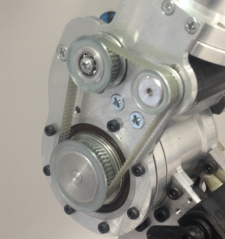
\includegraphics[scale=.5]{ElbowAssembly}}
\end{minipage}
\hfill
\begin{minipage}[h]{0.49\linewidth}
    \center{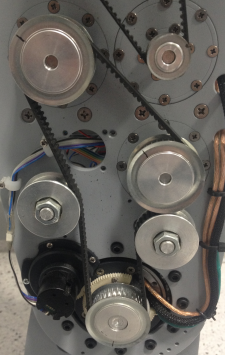
\includegraphics[scale=.5]{knee}}
\end{minipage}}
\caption{Elbow and knee assemblies}
\label{img:joints}
\end{figure}

Main controller board built on top of 3 STM 32F107 microcontrollers, minor
driver controllers are built on STM 32F103 microcontrollers. Both types use
Cortex-M3 ARM cpu and provide softwatre interfaces for hardware interaction. 

Joint drives are accompanied by two encoders. Main encoder provides absolute
position data with quite a broad error rate, supplementary encoder provides
relative motion data for more accurate position estimation.

IMU is Analog Devices ADIS 16400, placed just in center of mass to minimize
number of transforms required for calculations. There are also CCD camera,
speakers and microphone.

There is a frame on the chest, that allows to mount additional sensors like
kinect or laser rangefinders, however there no holes in plastic cover for that.
There also two small displays in head mount, that mimic eyes and eyebrows.

\subsection{Power}
Robot can run on internal LiFePo cells assembly as well as on external power
source. Main voltage is 48V, individual parts operate with 6V, 8V and 12V.
Autonomous work time depends on many factors, but typically robot can run for a
30-40 minutes.
 
\subsection{Wrist and palm assembly}
Robot has palms with five fingers one opposite to another four. All
finger motors are placed in wrist-elbow section, movement of motor translated to finger
via system of strings(fig. \ref{img:wrist}). This system limits wrist rotation,
but makes whole assembly significantly lighter. Our current arm is capable to grab objects like
tennis ball, Rubik`s cube or coffee cup, however there are
another types of hands under development - palm assembly is under
constant development.

\begin{figure}[h]
\framebox{
\begin{minipage}[h]{0.49\linewidth}
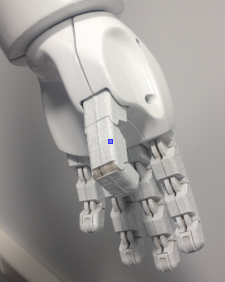
\includegraphics[scale=0.5]{palm}
\end{minipage}
\hfill
\begin{minipage}[h]{0.49\linewidth}
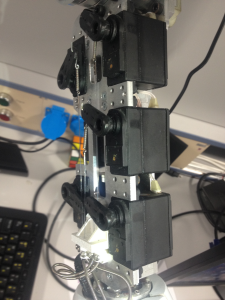
\includegraphics[scale=0.5]{wrist}
\end{minipage}}
\caption{Palm assembly}
\label{img:wrist}
\end{figure}  

\subsection{Control PC and communication bus}
Internal communications are built on ethernet. Controller boards are connected
via Zigbee interfaces to switch, which governs internal network as shown
in \ref{img:ethernet}.

There is also an embedded PC placed in back of robot and connected to same internal LAN. PC is
Avalue ECM-QM78 with Intel Core i7-4700EQ CPU and 8GB RAM, capable to carry out
performance-demanding sensor-processing tasks. However, there is an option to
connect any other PC via ethernet interface.

   \begin{figure}[thpb]
      \centering
      \framebox{
        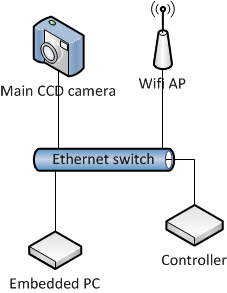
\includegraphics[scale=.5]{EthernetBus}
      }
      \caption{Internal network scheme}
      \label{img:ethernet}
   \end{figure}
   
\section{SOFTWARE}

Main software interface for controller boards is UDP with specially formed
datagrams. There two types of datagrams - one is for commands transmission,
another returns sensors data. Both UDP streams
are independent.

Datagram types encapsulate specific byte array, which encode movement
commands and sensors data, so one can easily subscribe interact with robot via
standard socket interface libraries.

We already have a set of ROS packages including urdf description for Rviz,
moveIt support for whole robot and hand assemblies, gazebo support, neural
network and cascade-based vision, speech packets and set of drivers for direct
robot interaction.

\section{CONCLUSIONS}

This paper presented a humanoid robot AR-600, its hardware design and
specifications. Drivers and software that work under ROS framework are
also described.

The next generation of the robot, named AR-600E (fig. \ref{img:ar600e}) is
expected to be available soon and this will be more powerful, more lightweight,
more autonomous system.

Future work includes releasing ROS support packages for public use, development
of full-body motion planning with MoveIt (including bipedal walking). Switching
from position controller to torque controller is also a priority that
will enable more gentle and human-like moves. 

We hope AR-600 and his successor AR-600E will be among top humanoid platforms
used in robotics research and capable of working alongside with humans.

\begin{figure} [thpb]
      \centering
      \framebox{
      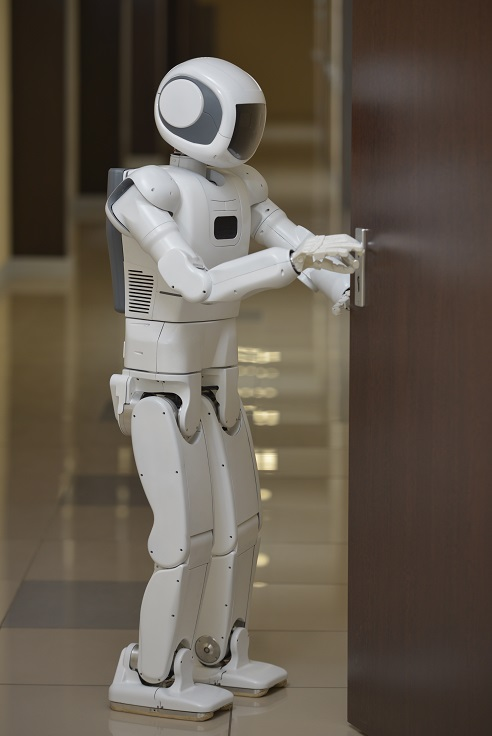
\includegraphics[scale=1]{ar600e}}
      \caption{AR-600E robot.}
      \label{img:ar600e}
\end{figure}

\addtolength{\textheight}{-12cm}   % This command serves to balance the column lengths
                                  % on the last page of the document manually. It shortens
                                  % the textheight of the last page by a suitable amount.
                                  % This command does not take effect until the next page
                                  % so it should come on the page before the last. Make
                                  % sure that you do not shorten the textheight too much.

%%%%%%%%%%%%%%%%%%%%%%%%%%%%%%%%%%%%%%%%%%%%%%%%%%%%%%%%%%%%%%%%%%%%%%%%%%%%%%%%



%%%%%%%%%%%%%%%%%%%%%%%%%%%%%%%%%%%%%%%%%%%%%%%%%%%%%%%%%%%%%%%%%%%%%%%%%%%%%%%%



%%%%%%%%%%%%%%%%%%%%%%%%%%%%%%%%%%%%%%%%%%%%%%%%%%%%%%%%%%%%%%%%%%%%%%%%%%%%%%%%


\begin{thebibliography}{99}

\bibitem{c1} Android Techniques. URL: http://en.npo-at.com/
\bibitem{c2} ROS
\bibitem{c3} MoveIt


\end{thebibliography}


\end{document}
